% CA report (CP4101 continuous assessment, 10-15 pages).
% Build: latexmk -pdf -outdir=build ca.tex
% The full dissertation draft (main.tex, chapters/) is untouched; this file reuses
% its preamble, cover, title page and bibliography.
\documentclass[12pt]{report}
\usepackage[T1]{fontenc}
\usepackage[utf8]{inputenc}
\usepackage[a4paper, margin=1in]{geometry}
\usepackage{tabto}
\usepackage{float}
\usepackage{color}   %May be necessary if you want to color links
\usepackage{hyperref}
\usepackage[toc,page,title,titletoc]{appendix}
% https://tex.stackexchange.com/questions/51434/biblatex-citation-order
\usepackage{amsmath, amssymb, amsthm}
\newtheorem{Definitions}{Definition}[chapter]
\usepackage[
    backend=biber,
    style=apa,
    sorting=nyt
]{biblatex}
\addbibresource{cite.bib}
\usepackage[parfill]{parskip}
\hypersetup{
    colorlinks=true, %set true if you want colored links
    linktoc=all,     %set to all if you want both sections and subsections linked
    linkcolor=blue,  %choose some color if you want links to stand out
    citecolor=black,
    filecolor=black,
    linkcolor=black,
    urlcolor=black
}
\usepackage{multirow}
\usepackage{array}
\usepackage{siunitx} % For aligning numbers by decimal point
\usepackage{booktabs} % For better-looking horizontal separators
\usepackage{graphicx}
\usepackage[table,xcdraw]{xcolor}
\graphicspath{ {images/} }
\usepackage{minted}
\usepackage{mdframed}
\definecolor{bg}{rgb}{0.95,0.95,0.95}
\usepackage{enumitem}
\newcommand{\myparagraph}[1]{\paragraph{#1}\mbox{}\\}

\usepackage{times}
\usepackage{setspace} % Include the setspace package
\onehalfspacing % Set line spacing to 1.5
% \linespread{1.15}

\usepackage{listings}

% Setup the listings package
\lstset{
  basicstyle=\small\ttfamily, % The style of the code
  numbers=left,         % Where to put the line numbers
  numbersep=5pt,        % How far the line numbers are from the code
  tabsize=2,            % Sets default tab size to 4 spaces
  extendedchars=true,
  breaklines=true,      % Sets automatic line breaking
  frame=single,         % Adds a frame around the code
  breakatwhitespace=true
}

\usepackage{algorithm}
\usepackage{algpseudocode}

\usepackage{tikz}
\usetikzlibrary{tikzmark, arrows.meta}

\renewenvironment{abstract}
 {\small
  \begin{center}
  \bfseries \abstractname\vspace{-.5em}\vspace{0pt}
  \end{center}
  \addcontentsline{toc}{chapter}{\abstractname} % Add to ToC
  \list{}{%
    \setlength{\leftmargin}{0pt}
    \setlength{\rightmargin}{\leftmargin}%
  }%
  \item\relax}
 {\endlist}

\newenvironment{acknowledgements}
 {\small
  \begin{center}
  \bfseries Acknowledgements\vspace{-.5em}\vspace{0pt}
  \end{center}
  \addcontentsline{toc}{chapter}{Acknowledgements} % Add to ToC
  \list{}{%
    \setlength{\leftmargin}{0pt}
    \setlength{\rightmargin}{\leftmargin}%
  }%
  \item\relax}
 {\endlist}

 \renewcommand\tab[1][10mm]{\hspace*{#1}}

\newcommand{\projecttype}{B.Comp. Dissertation}
\newcommand{\authorname}{Ansel Chong}
\newcommand{\projecttitle}{Automated Agentic AI}
\newcommand{\academicyear}{2026/2027}


% Numbered findings, in the style of the paper's takeaway boxes.
\newcounter{takeaway}
\newenvironment{takeaway}[1]{%
  \refstepcounter{takeaway}%
  \begin{mdframed}[backgroundcolor=bg, linewidth=0pt, innertopmargin=6pt,
    innerbottommargin=6pt, skipabove=8pt, skipbelow=8pt]%
  \textbf{Takeaway~\thetakeaway: #1}\par\smallskip\noindent\ignorespaces}%
  {\end{mdframed}}


% A short report: compact chapter headings that do not start a new page.
\usepackage{titlesec}
\titleclass{\chapter}{straight}
\titleformat{\chapter}{\Large\bfseries}{\thechapter}{0.8em}{}
\titlespacing*{\chapter}{0pt}{14pt}{8pt}
\renewcommand{\projecttype}{B.Comp. Dissertation\\[2mm]Continuous Assessment Report}
\renewcommand{\projecttitle}{Automated Agentic AI\\[5mm]
  {\Large Provider-Selective Distillation: A Curriculum\\over Teachers and Domains}}

\begin{document}

\input{cover.tex}
\newgeometry{left=3cm,right=3cm,top=3cm,bottom=3cm}
\begin{titlepage}
    {\centering
    {\large \projecttype}
    \vfill
    {\LARGE\bfseries \projecttitle\par}
    \vspace{2cm}
    {\large By\par \authorname}
    \vfill
    {\normalsize Department of Computer Science\par
    School of Computing\par
    National University of Singapore\par}
    \vspace{1cm}
% Bottom of the page
    {\normalsize \academicyear\par}
    }
    \vspace{1cm}
    Project ID: H148650 \par
    Advisor: Professor Low Kian Hsiang \par
    \vspace{1cm}
    Deliverables: \par
    \begin{list}{\quad}{}
        \item Report: 1 Volume
    \end{list}
\end{titlepage}
\restoregeometry
\pagebreak

\pagenumbering{roman}
\begin{abstract}
\noindent
Small language models are increasingly trained by distilling from larger models, and
several such models are often available. The student must then decide which one to learn
from, on which domain, and when; the common default is the strongest throughout. We treat
this as a curriculum learning problem over pairs of provider and domain, which we term
provider-selective distillation: the next pair is chosen from the progress the student
actually makes. This semester we studied a first version of the problem, with text-only
providers and a price on every query, on a testbed with a 1.5B-parameter student, five
providers and three domains with checkable answers. We
find that providers of very different strength teach at a similar rate per gradient step,
so price decided value and the strongest provider was the worst single
choice. A selector that learns where progress happens matches the best single provider
(test utility 0.500 against 0.494) without being told which one it is. Learning was
confined to one domain and was unstable. These findings lead us to refine the problem: we
remove the budget, give the student the providers' token probabilities, and aim for a
framework in which a student can pass its teachers.

\vspace{5mm}
Subject Descriptors:
\begin{list}{\quad}{}
    \item I.2.6 Learning
    \item I.2.7 Natural Language Processing
    \item G.3 Probability and Statistics
\end{list}

Keywords: \\
\tab On-policy distillation, curriculum learning, multi-teacher distillation,
multi-armed bandits

Implementation Software and Hardware:
\begin{list}{\quad}{}
    \item Python 3.12, PyTorch, vLLM, TRL, PEFT, Math-Verify, bubblewrap
    \item NVIDIA L40 GPUs (shared server); SoC Slurm cluster (A100, H100)
\end{list}
\end{abstract}
\pagebreak


\setcounter{tocdepth}{1}
\tableofcontents
\clearpage

\pagenumbering{arabic}
\setcounter{page}{1}
\chapter{Introduction}
\label{ca:chap:intro}

Much of the knowledge a practitioner would like to train on is no longer available as
data. Hospitals, banks and firms rarely release their datasets, but they increasingly
expose models trained on them, through an interface or as open weights. For anyone training
a small language model, the resource at hand is therefore less often a dataset and more
often a set of models to learn from, each with its own competence. On-policy distillation,
in which the student learns from its own responses as scored by a teacher
\autocite{agarwal_gkd_2024,gu_minillm_2024}, is a natural way to learn from such models.

Deciding what a learner should practise next is the subject of curriculum learning
\autocite{bengio_curriculum_2009}. Automated curricula treat the decision as a bandit
problem in which a task is rewarded by the progress the learner makes on it
\autocite{graves_curriculum_2017,matiisen_tscl_2017}, and the idea has recently been
applied to the fine-tuning of language models, with problem categories as the tasks
\autocite{chen_sec_2025}. Distillation from several models adds a second decision to the
curriculum: not only what to practise, but whom to learn it from. The usual default is the
strongest model. However, small models (3B parameters or fewer) often learn more from
smaller teachers than from strong reasoners \autocite{li_learnability_gap_2025}, and a
larger teacher does not necessarily give a better student \autocite{guo_lada_2026}. We
therefore study a curriculum over pairs of provider and domain, which we term
provider-selective distillation.

\begin{mdframed}[backgroundcolor=bg, linewidth=0pt, innertopmargin=8pt,
  innerbottommargin=8pt]
Given several white-box providers and different domains, how should a student decide whom
to ask, about what, and when?
\end{mdframed}

This report covers the first version of the problem that we studied. In it the providers
are black-box, returning only text, and every query has a price, so the curriculum must
fit a fixed budget. The findings of that study, together with feedback on the project, led
to the statement above, which removes the budget and lets the student read the providers'
token probabilities. Section~\ref{ca:sec:refined} explains the change.

\begin{figure}[htbp]
\centering
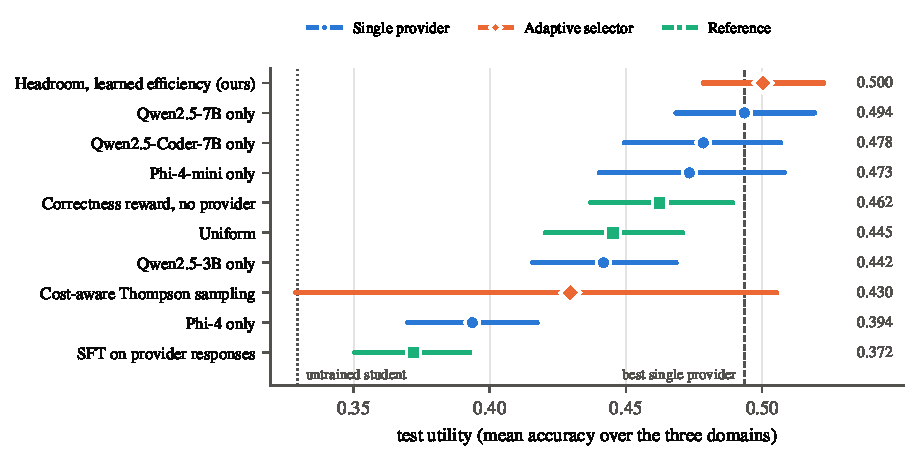
\includegraphics[width=0.95\linewidth]{ca_teaser.pdf}
\caption{At an equal budget of 2,400 price units, the most expensive provider (Phi-4) is
the worst single teacher, and our selector, which learns where progress happens, matches
the best single provider without being told which one it is. Points are test utility
averaged over three seeds; bars are 95\% bootstrap intervals.}
\label{ca:fig:teaser}
\end{figure}

The problem differs from online data mixing \autocite{albalak_odm_2023} and LLM routing
\autocite{ong_routellm_2025} in one essential way: every choice changes the student, and
with it the value of every provider at the next decision. So far, we have (1) built a
reproducible testbed with priced black-box providers, including a corrupted one; (2)
measured the value of each provider directly, by training from shared student checkpoints
on one provider at a time; and (3) designed selectors that learn from the student's
progress and compared them with fixed allocations. Figure~\ref{ca:fig:teaser} summarises
the main result. Cheap providers teach about as fast per gradient step as expensive ones,
so under a budget price decides value (Takeaway~\ref{ca:tk:price}). Our selector reaches
the highest test utility of any condition, 0.500 against 0.494 for the best single
provider, but the difference is within noise (Takeaway~\ref{ca:tk:h3}).

\section{Objectives and Scope}
\label{ca:sec:objectives}

This semester had four objectives: to build the testbed; to test whether the best provider
differs by domain (H1) and changes during training (H2); to design selectors and test
whether adaptivity beats the best fixed allocation (H3); and to explain where learning
happens and what the selectors choose. Next semester's objective is a training framework
for the refined problem: a student that learns from several providers of its own model
family, with their token probabilities, efficiently enough to make progress on every
domain and to pass its teachers. Strategic providers, providers that learn from the
student and formal privacy guarantees are out of scope. Tasks are single-turn with
checkable answers, so that rewards are cheap and need no learned judge.

\chapter{Literature Review}
\label{ca:chap:lit}

\section{Curriculum learning}

Curriculum learning orders training examples from easy to hard by a fixed measure of
difficulty \autocite{bengio_curriculum_2009}, and self-paced learning lets the model's own
loss set the order \autocite{kumar_selfpaced_2010}. Automated curricula remove the fixed
measure: a bandit chooses the next task and is rewarded by the learner's progress on it
\autocite{graves_curriculum_2017,matiisen_tscl_2017}, and Prioritized Level Replay revisits
the tasks on which a reinforcement learning agent can still improve
\autocite{jiang_plr_2021}. For language models, Online Data Mixing reweights data domains
with an EXP3 bandit on training loss \autocite{albalak_odm_2023,auer_exp3_2002}, and the
Self-Evolving Curriculum chooses problem categories during reinforcement learning
fine-tuning by the size of the advantages they produce \autocite{chen_sec_2025}. All of
these choose what to practise, from fixed tasks or datasets. In contrast, our curriculum
also chooses whom to learn from, and the sources are models whose usefulness depends on the
student.

\section{On-policy distillation}

GKD and MiniLLM train the student on its own samples under a divergence to the teacher
\autocite{agarwal_gkd_2024,gu_minillm_2024}, which avoids the compounding errors of
training on the teacher's samples \autocite{ross_dagger_2011} but needs the teacher's
next-token probabilities over a shared vocabulary. Cross-tokenizer losses relax the shared
vocabulary \autocite{boizard_uld_2025,patino_gold_2025}, but any fixed alignment discards
supervision where segmentations disagree \autocite{sun_simct_2026}. Black-box methods turn
the teacher's text into a reward instead: a discriminator in GAD \autocite{ye_gad_2025},
a rubric checked by a verifier in ROPD \autocite{fang_ropd_2026}, or similarity to teacher
continuations in OmniOPD \autocite{zhou_omniopd_2026}. FedTOPS shows, with one teacher and
several clients, that the student's progress changes what it can next learn from that
teacher \autocite{chen_fedtops_2026}. All of these assume one teacher consulted on every
prompt. Our work asks which of several teachers to consult.

\section{Multi-teacher distillation}

A teacher that is too strong can teach worse than a weaker one, which motivated inserting a
mid-sized teacher assistant between the two \autocite{mirzadeh_ta_2020} and was observed
again for small language models \autocite{li_learnability_gap_2025}. With several teachers,
MOPD routes each prompt to a specialist teacher for its domain \autocite{ma_mopd_2026},
TrustMOPD weights teachers per token by a reliability proxy
\autocite{sun_trustmopd_2026}, and MAD-OPD weights them by their confidence after a debate
\autocite{wang_madopd_2026}. RL-KD learned per-instance teacher weights with reinforcement
learning, but for off-policy distillation \autocite{yuan_rlkd_2021}. Federated distillation
likewise combines the predictions of several parties
\autocite{li_fedmd_2019,lin_feddf_2020,fan_fedmkt_2025}. In these methods the routing or
weighting rule is fixed by domain labels or by a property of the teachers. In contrast, our
selectors learn the rule from the student's realised progress.

\section{Bandits whose arms change the learner}

Bandit theory handles budgets \autocite{badanidiyuru_bwk_2013}, rewards that drift
\autocite{garivier_ducb_2011} and context \autocite{li_linucb_2010}, and rotting bandits let
an arm's reward decay as it is pulled \autocite{levine_rotting_2017}. None of them models
our case, where pulling any arm changes the student and therefore the value of every other
arm. Table~\ref{ca:tab:gap} summarises the gap.

\begin{table}[htbp]
\centering
\footnotesize
\setlength{\tabcolsep}{3pt}
\begin{tabular}{@{}lccccc@{}}
\toprule
\textbf{Method} & \textbf{Several} & \textbf{On-policy} & \textbf{Chooses} &
  \textbf{Chooses} & \textbf{Learned from} \\
 & \textbf{teachers} & \textbf{distillation} & \textbf{teacher} & \textbf{domain} &
  \textbf{progress} \\
\midrule
TSCL \autocite{matiisen_tscl_2017} & -- & -- & -- & \checkmark & \checkmark \\
Self-Evolving Curriculum \autocite{chen_sec_2025}        & -- & -- & -- & \checkmark & \checkmark \\
Online Data Mixing \autocite{albalak_odm_2023}           & -- & -- & -- & \checkmark & \checkmark \\
GKD \autocite{agarwal_gkd_2024}                          & -- & \checkmark & -- & -- & -- \\
MOPD \autocite{ma_mopd_2026}                             & \checkmark & \checkmark & \checkmark & -- & -- \\
TrustMOPD \autocite{sun_trustmopd_2026}                  & \checkmark & \checkmark & \checkmark & -- & -- \\
\midrule
This project                                             & \checkmark & \checkmark & \checkmark & \checkmark & \checkmark \\
\bottomrule
\end{tabular}
\caption{Curriculum methods choose what to practise and multi-teacher methods choose whom
to learn from, but no existing method chooses both from the student's own progress.
TSCL is the teacher-student curriculum. Learned from progress: the choice is revised during training from a signal of how much the
student is learning; MOPD and TrustMOPD choose the teacher by a fixed rule.}
\label{ca:tab:gap}
\end{table}

\chapter{Preliminaries}
\label{ca:chap:prelim}

\section{Notation and Problem Statement}
\label{ca:sec:problem}

A student policy $\pi_\theta$ can learn from $K$ providers $M_1, \dots, M_K$. Prompts
come from $D$ domains $\mathcal{X}_1, \dots, \mathcal{X}_D$, and the student's utility
$U(\theta)$ is its mean accuracy over held-out sets, one per domain. Training proceeds in
rounds. In round $t$ a selector chooses an arm $a_t = (k_t, d_t)$, a provider and a
domain, and the student is updated on a batch $S_{k_t,d_t}$ of $b$ prompts from
$\mathcal{X}_{d_t}$ under the supervision of $M_{k_t}$. The sequence of arms is the
curriculum. The selector sees only the student's accuracy on a selection set that is
disjoint from the test sets, and it should make $U(\theta_t)$ rise as fast and as far as
possible. The quantity it must estimate is the marginal value of an arm at the current
state,
\[
  g(k, d; \theta) =
  \mathbb{E}\big[\, U\big(\operatorname{Update}(\theta, S_{k,d})\big) - U(\theta) \,\big].
\]
If $g$ did not depend on $\theta$, the problem would be an ordinary bandit. Because every
update changes $\theta$, the values drift as a result of the selector's own choices.

\paragraph{The budgeted, black-box version.} All experiments in this report use the first
version of the problem. Provider $M_k$ is a sampling oracle that returns a text response to
a prompt at price $c_k$, a round on arm $(k, d)$ is charged $b\,c_k$, and training stops
when a budget $B$ is spent. The selector then maximises $\mathbb{E}[U(\theta_\tau)]$
subject to $\sum_{t \le \tau} b\,c_{k_t} \le B$, and the relevant quantity is the marginal
value per unit of cost, $v(k, d; \theta) = g(k, d; \theta) / (b\,c_k)$.

\paragraph{Hypotheses.} The problem is worth solving only if provider value varies in this
way, so we test three hypotheses in order. H1 (non-dominance): at a fixed student state,
the provider of highest marginal value differs across domains. H2 (state dependence):
within a domain, the provider of highest marginal value changes during training. H3
(adaptivity pays): an adaptive selector reaches higher test utility than the best static
allocation at equal budget. H1 alone would justify a fixed allocation per domain, H2 makes
adaptive selection necessary, and H3 makes it worthwhile. A negative H2 is also useful: it
would show that an allocation fixed before training is enough.

\section{Black-Box On-Policy Distillation}
\label{ca:sec:opd}

\paragraph{Agreement reward.} Each provider answered every prompt four times, and every
response is reduced to a canonical final answer (an expression's value, a normalised maths
answer, or a program's outputs on the test inputs). Let $n_k(z; x)$ count how many of
provider $k$'s answers to prompt $x$ equal $z$. A student response with answer $z$ receives
\[
  r_k(z; x) = \frac{n_k(z; x)}{\max_{z'} n_k(z'; x)},
\]
or 0 if it has no valid answer. If the provider answered $\{18, 18, 18, 22\}$, the student's
answers 18, 22 and 7 receive 1, $1/3$ and 0. No ground truth enters training.

\paragraph{Update.} The student samples $G = 8$ responses to each of $b = 8$ prompts. Each
reward is turned into a group-relative advantage by subtracting the mean of its prompt's
eight rewards and dividing by their standard deviation, as in GRPO
\autocite{shao_deepseekmath_grpo_2024}, and the student takes one policy-gradient step.
A prompt whose eight answers are identical would give every response the same reward and
no gradient, so it is skipped before the provider is consulted and is not charged.

\paragraph{The ceiling.} The expected reward on a prompt is highest when the student always
gives the provider's most common answer. A student that fully learned from provider $k$
would therefore be right exactly where that answer is right. We call this accuracy the
provider's ceiling $\mu_{k,d}$ and use it, rather than single-response accuracy, as the
measure of a provider's quality as a teacher. The ceiling is a per-prompt argument, not a
hard limit: in our pilot the student passed two providers' ceilings on Countdown by applying
what it learned on prompts the provider got right to prompts it got wrong.

\chapter{Testbed and Selectors}
\label{ca:chap:testbed}

\section{Experimental Setup}
\label{ca:sec:setup}

\paragraph{Domains.} We use three domains whose answers a program can check: three-number
Countdown puzzles \autocite{patino_gold_2025}, MATH problems at difficulty levels 3 to 5
\autocite{hendrycks_math_2021}, and Python function-writing problems from KodCode
\autocite{xu_kodcode_2025}, kept only if their reference solution passes its tests in our
sandbox. Each domain has a 2,000-prompt training pool, a 500-prompt selection set that
feeds the selector, and a 500-prompt test set used only for final results. Generated code
runs in a bubblewrap sandbox with no network and a read-only file system.

\paragraph{Student.} The student is Qwen2.5-1.5B-Instruct \autocite{qwen_qwen25_2024},
trained through a rank-16 LoRA adapter \autocite{hu_lora_2022}. Before training it scores
0.208 on Countdown, 0.474 on MATH and 0.396 on code on the selection set.

\paragraph{Providers.} Nine open models were screened on 200 prompts per domain and five
were kept (Table~\ref{ca:tab:pool}). They run locally but are reached only through a text
interface, so black-box access is enforced rather than assumed. The pool has a strong and
expensive model, a mid-priced generalist, a code specialist, a cheap model the student can
catch up with, and a cheap model from a second family, which separates any effect of
sharing the student's family from an effect of price. A sixth provider is a copy of Phi-4
at the same price whose answers are corrupted on 30\% of prompts.

\begin{table}[htbp]
\centering
\small
\begin{tabular}{@{}llrccc@{}}
\toprule
 & & & \multicolumn{3}{c}{\textbf{Ceiling $\mu_{k,d}$}} \\
\cmidrule(l){4-6}
\textbf{Provider} & \textbf{Size} & \textbf{Price $c_k$} & \textbf{Countdown} &
  \textbf{MATH} & \textbf{Code} \\
\midrule
Phi-4 \autocite{abdin_phi4_2024}                 & 14.7B & 2.92 & 0.874 & 0.804 & 0.686 \\
Qwen2.5-7B \autocite{qwen_qwen25_2024}           & 7.6B  & 1.00 & 0.810 & 0.750 & 0.580 \\
Qwen2.5-Coder-7B \autocite{hui_qwen25coder_2024} & 7.6B  & 0.98 & 0.620 & 0.678 & 0.612 \\
Qwen2.5-3B \autocite{qwen_qwen25_2024}           & 3.1B  & 0.50 & 0.538 & 0.690 & 0.462 \\
Phi-4-mini \autocite{microsoft_phi4mini_2025}    & 3.8B  & 0.84 & 0.616 & 0.618 & 0.558 \\
Phi-4, degraded                                  & 14.7B & 2.92 & 0.614 & 0.532 & 0.492 \\
\bottomrule
\end{tabular}
\caption{The strongest provider is also the most expensive. Price is GPU time per response
relative to Qwen2.5-7B; the ceiling is the accuracy of the provider's most common answer
over its four cached responses on the selection set.}
\label{ca:tab:pool}
\end{table}

\paragraph{Prices and cache.} A provider's price is the GPU time it needs to produce one
response, relative to Qwen2.5-7B, measured during screening and fixed before training.
Long-winded providers therefore cost more, as under per-token pricing. Each provider
answered every pool and selection prompt four times, once; runs read these cached answers,
which makes them reproducible and the measurements of Section~\ref{ca:sec:branching}
affordable.

\paragraph{Training and evaluation.} Every run has a budget of $B = 2{,}400$ price units
and a cap of 400 rounds. The selector chooses an arm once per block of 10 rounds, after
which the student is evaluated greedily on 256 selection prompts per domain. Final students
are evaluated on all 1,500 test problems. Every condition is run with three seeds, and
intervals are 95\% bootstrap intervals over seeds and test items.

\section{Selectors}
\label{ca:sec:selectors}

\paragraph{Headroom with learned efficiency (ours).} The selector scores each arm by how
far the student is below the provider's ceiling, scaled by a learned estimate of how much
accuracy that headroom buys, and divided by price:
\[
  \hat{v}(k, d) = \max\big(\hat{g}_{k,d},\, 0\big) \cdot
                  \frac{\max\big(\mu_{k,d} - \alpha_d,\ 0.05\big)}{c_k},
\]
where $\alpha_d$ is the student's current selection accuracy on domain $d$. The efficiency
$\hat{g}_{k,d}$ is the realised accuracy gain per round per unit of headroom, pooled per
domain, shrunk towards the domain's estimate and discounted by 0.95 per block, so that a
domain where no provider produces progress is learned to be unproductive for all of them at
once. With probability 0.1 the selector plays a random arm instead, so every arm keeps
being observed.

\paragraph{Cost-aware Thompson sampling.} A model-free comparison that keeps a discounted
Gaussian posterior over each arm's gain per round and plays the arm with the largest
sampled gain divided by price \autocite{xia_budgeted_ts_2015,raj_dts_2017}.

\paragraph{Reference policies.} Uniform allocation over all 18 arms; each real provider
alone, with domains in rotation; a control trained on ground-truth correctness with no
provider and no cost for 200 rounds, which shows what providers add beyond the labels; and
supervised fine-tuning (SFT) on provider responses bought with the same budget, which shows
what learning on-policy adds.

\section{Measuring Marginal Value}
\label{ca:sec:branching}

We measure $v(k, d; \theta)$ directly by branching. The uniform run of each seed saves
checkpoints at 25, 50 and 75\% of its budget, and the untrained student serves as the 0\%
checkpoint. From each checkpoint, a branch trains on a single arm for 20 rounds and is then
evaluated on the full selection set; marginal value is the change in mean selection
accuracy divided by the budget the branch spent. With 6 providers, 3 domains, 4 checkpoints
and 3 seeds this gives 216 branches. Branches from the same checkpoint and seed share the
adapter, the prompt order and the sampling seeds, so comparisons between providers are
paired.

\section{Design Decisions}
\label{ca:sec:decisions}

Table~\ref{ca:tab:decisions} lists the choices that most shape the results, the
alternatives we considered, and the evidence behind each choice.

\begin{table}[htbp]
\centering
\footnotesize
\renewcommand{\arraystretch}{1.1}
\begin{tabular}{@{}>{\raggedright\arraybackslash}p{2.7cm}
                >{\raggedright\arraybackslash}p{3.9cm}
                >{\raggedright\arraybackslash}p{8.3cm}@{}}
\toprule
\textbf{Decision} & \textbf{Alternatives} & \textbf{Reason for the choice} \\
\midrule
Black-box agreement reward & Logit-based on-policy distillation across tokenizers &
  Cross-tokenizer distillation recovered 0.14 of the teacher gap against 0.66 with a shared
  tokenizer, and its hybrid variant collapsed (Takeaway~\ref{ca:tk:blackbox}). \\
Normalised vote share & Most-common-answer indicator; raw vote share; rubric with a verifier &
  Carried as much learning signal as ground truth on MATH and code in screening, kept signal
  on Countdown where providers often give invalid answers, and needs no extra model. \\
Ceiling as provider quality & Single-response accuracy; agreement with other providers &
  It is where the reward points the student. Agreement with peers was label-free but
  favoured the Qwen family, which made up most of the pool. \\
Countdown (3 numbers), MATH 3--5, KodCode & GSM8K; MBPP; 4-number Countdown &
  GSM8K was saturated (all large providers scored 94--97\%), MBPP had too few problems, and
  the student solved 0.8\% of 4-number puzzles, leaving almost no gradient. \\
Price = GPU time per response & Parameter count; hosted API prices &
  Measured on our hardware and fixed before training, and captures verbosity: one candidate
  repeated itself until the length limit. \\
Corrupt whole prompts in the degraded provider & Corrupt each response independently &
  Independent corruption at 30\% lowered the ceiling by only 8\%, because the majority
  usually survives; per-prompt corruption lowers it by 30\%. \\
\bottomrule
\end{tabular}
\caption{Main design decisions and their evidence.}
\label{ca:tab:decisions}
\end{table}

\chapter{Findings So Far}
\label{ca:chap:findings}

All three hypotheses have now been run once at full scale, with three seeds. This chapter
reports what we have found and how confident each finding is.

\section{Text-Only Supervision Avoids the Tokenizer Cost}
\label{ca:sec:motivating}

The black-box assumption gives up the teacher's token probabilities. To see what those are
worth, we ran on-policy distillation from Qwen3-4B-Instruct on Countdown with three
students, each first fine-tuned to the same starting accuracy of about 0.38
(Table~\ref{ca:tab:motivating}). Recovery $R$ is the fraction of the gap between that
starting point and the teacher (0.713) that distillation closed.

\begin{table}[htbp]
\centering
\small
\begin{tabular}{@{}llllc@{}}
\toprule
\textbf{Student} & \textbf{Tokenizer} & \textbf{Loss} & \textbf{Accuracy} & $R$ \\
\midrule
Qwen2.5-1.5B & shared    & exact logits (GKD)         & 0.379 $\to$ 0.600 & 0.66 \\
Qwen2.5-1.5B & shared    & cross-tokenizer loss (ULD) & 0.379 $\to$ 0.487 & 0.32 \\
OLMo-2-1B    & different & cross-tokenizer loss (ULD) & 0.381 $\to$ 0.426 & 0.14 \\
OLMo-2-1B    & different & GOLD hybrid                & 0.381 $\to$ 0.035 & collapsed \\
SmolLM2-1.7B & different & GOLD hybrid                & 0.375 $\to$ 0.000 & collapsed \\
\bottomrule
\end{tabular}
\caption{Each step away from a shared tokenizer roughly halves what distillation recovers,
and the hybrid cross-tokenizer loss collapses. Countdown, 200 steps, 1,000 test puzzles;
the first OLMo-2 GOLD run was stopped at step 110.}
\label{ca:tab:motivating}
\end{table}

The cross-tokenizer loss alone halved recovery on a shared tokenizer (paired difference
$+0.113$, 95\% interval $[+0.091, +0.136]$), and a real mismatch halved it again. The GOLD
hybrid loss collapsed on both cross-tokenizer students while its value kept falling: it
forced OLMo-2 into the teacher's single-digit number tokens, which broke its arithmetic, and
it let SmolLM2 emit newlines to the length limit.

\begin{takeaway}{Text-Only Supervision Is the Safer Choice}
\label{ca:tk:blackbox}
Logit-level supervision across model families is both lossy and fragile, so a reward
computed from the teacher's text is a sound basis for learning from heterogeneous providers.
\end{takeaway}

\section{Selectors Need Feedback from Realised Gains}
\label{ca:sec:pilot}

We first ran every condition once (seed 0, 14.4 GPU-hours) to test the pipeline. The
original headroom selector, which scored arms by headroom over price alone, made the switch
it predicted before training, from Qwen2.5-3B to Qwen2.5-7B on Countdown once the student
passed an accuracy of about 0.27. It then spent 320 of its 400 rounds on MATH, where the
headroom never shrank because nothing was learned. The original Thompson sampling divided
each noisy gain by its cost before learning, which shrinks the noise of expensive arms
towards zero, and it spent 55\% of its budget on the degraded provider. A five-times-higher
learning rate did not help MATH or code and cut the Countdown gain from $+0.280$ to
$+0.098$. We kept the learning rate, added the learned efficiency to the headroom selector,
and made Thompson sampling apply the price only when choosing.

\begin{takeaway}{Headroom Is Not Enough}
\label{ca:tk:feedback}
A domain can have large headroom and no learnability, so a selector must learn from the
progress it actually observes, and noisy gains must not be divided by cost before they are
averaged.
\end{takeaway}

\section{Price, Not Provider Identity, Decides Value (H1, H2)}
\label{ca:sec:h12}

Figure~\ref{ca:fig:mv} shows the marginal value of every provider on every domain at the
four checkpoints, from all 216 branches.

\begin{figure}[htbp]
\centering
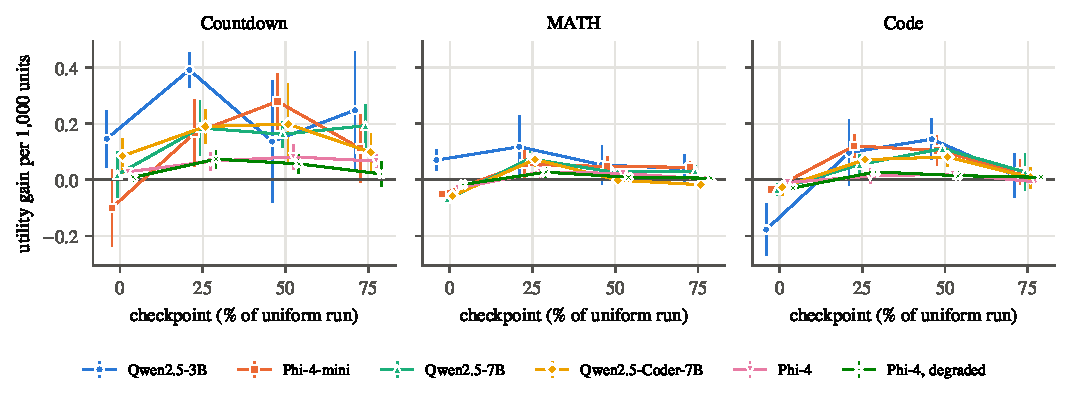
\includegraphics[width=\linewidth]{ca_marginal_value.pdf}
\caption{On Countdown, the cheapest provider usually gives the most progress per unit of
budget, and on MATH and code every provider gives almost none. Change in mean selection
accuracy after 20 rounds on one arm, per 1,000 price units; points are means over three
seeds, bars $\pm 1$ standard error, offset horizontally for legibility.}
\label{ca:fig:mv}
\end{figure}

\paragraph{Cheap providers lead per unit of budget.} On Countdown, the cheapest provider,
Qwen2.5-3B, has the highest mean marginal value at the 0, 25 and 75\% checkpoints, and
Phi-4-mini at 50\%; Qwen2.5-3B is the best Countdown arm in 8 of the 12 combinations of seed
and checkpoint. Per round, without dividing by price, the providers are much closer. For
example, from the 25\% checkpoint all six raise mean utility by between 0.022 and 0.033 in
20 Countdown rounds. Phi-4 teaches no faster per round, to within noise, than providers that
cost a third as much. Its only lead is on code from the untrained student, where every
provider lowered utility and Phi-4 lowered it least. The only differences that are
significant in paired comparisons within a seed all involve Phi-4: at 25\%, Qwen2.5-3B beats
Phi-4 and its degraded copy on Countdown, and Phi-4-mini beats Phi-4 on code.

\begin{takeaway}{Price Decides Value}
\label{ca:tk:price}
Providers of very different strength teach a small student at a similar rate per gradient
step, so value per unit of budget is decided mainly by price, and the strongest provider is
rarely worth its price.
\end{takeaway}

\paragraph{H1 and H2 are below our current resolution.} Our decision rules, fixed before the
runs, require the leading provider's 95\% interval to clear its rival's; here these are
t-intervals over the three seeds. This never happens between the cheap and mid-priced
providers, at any checkpoint or in any domain. The leading provider does change between
checkpoints and domains, and the rankings are unstable: Kendall's $\tau$, which measures how
well the provider ranking at one checkpoint agrees with the ranking at the next, ranges from
$-0.60$ to $0.73$. But changes of that size are also what noise alone would produce.

\begin{takeaway}{H1 and H2 Remain Open}
\label{ca:tk:open}
Among the affordable providers, differences in marginal value are smaller than three seeds
of 20-round branches can detect, so we can neither confirm nor reject that the best
provider differs by domain or changes during training.
\end{takeaway}

\section{Adaptive Selection Matches the Best Provider (H3)}
\label{ca:sec:h3}

Table~\ref{ca:tab:h3} reports every condition on the test set.

\begin{table}[htbp]
\centering
\footnotesize
\setlength{\tabcolsep}{2.5pt}
\begin{tabular}{@{}lrccccc@{}}
\toprule
 & & \multicolumn{3}{c}{\textbf{Test accuracy}} & & \\
\cmidrule(l){3-5}
\textbf{Condition} & \textbf{Rounds} & \textbf{Countdown} & \textbf{MATH} & \textbf{Code} & \textbf{Utility [95\% CI]} & \textbf{Diff. [95\% CI]} \\
\midrule
Untrained student & -- & 0.218 & 0.434 & 0.336 & 0.329 & \\
\midrule
Qwen2.5-3B only & 400 & 0.555 & 0.418 & 0.352 & 0.442 [0.416, 0.468] & $-$0.052 [$-$0.083, $-$0.024] \\
Phi-4-mini only & 400 & 0.630 & 0.438 & 0.352 & 0.473 [0.440, 0.508] & $-$0.020 [$-$0.049, +0.009] \\
Qwen2.5-7B only & 364 & 0.698 & 0.423 & 0.360 & 0.494 [0.468, 0.519] & -- \\
Qwen-Coder-7B only & 360 & 0.656 & 0.421 & 0.358 & 0.478 [0.450, 0.507] & $-$0.015 [$-$0.032, +0.000] \\
Phi-4 only & 110 & 0.417 & 0.429 & 0.335 & 0.394 [0.370, 0.417] & $-$0.100 [$-$0.127, $-$0.073] \\
\midrule
Uniform & 223 & 0.556 & 0.437 & 0.343 & 0.445 [0.420, 0.471] & $-$0.048 [$-$0.068, $-$0.026] \\
Headroom, learned eff. & 368 & 0.711 & 0.435 & 0.355 & 0.500 [0.478, 0.523] & +0.007 [$-$0.011, +0.026] \\
Cost-aware Thompson & 400 & 0.508 & 0.435 & 0.346 & 0.430 [0.329, 0.505] & $-$0.064 [$-$0.165, +0.004] \\
\midrule
Correctness, no provider & 200 & 0.611 & 0.425 & 0.352 & 0.462 [0.437, 0.489] & $-$0.031 [$-$0.052, $-$0.011] \\
SFT on responses & -- & 0.373 & 0.421 & 0.322 & 0.372 [0.350, 0.393] & $-$0.122 [$-$0.144, $-$0.099] \\
\bottomrule
\end{tabular}
\caption{Test results of the main runs at budget $B = 2{,}400$, means over three seeds. Utility is the mean of the three domain accuracies. Intervals are 95\% bootstrap intervals over seeds and test items; the last column is the paired difference from the best single provider, Qwen2.5-7B. Rounds are gradient steps, capped at 400; SFT takes no rounds. Runs that reached the cap stopped before spending the whole budget; mean spend was lowest for Qwen2.5-3B alone (1,374 units).}
\label{ca:tab:h3}
\end{table}


\paragraph{Our selector matches but does not beat the best single provider.} The best
single provider is Qwen2.5-7B, with test utility 0.494. Our selector reaches 0.500, the
highest of any condition and the most consistent across seeds (0.503, 0.498 and 0.500), but
its paired advantage of $+0.007$ has a 95\% interval from $-0.011$ to $+0.026$. It learned
what the pilot version could not: it spent 38 to 58\% of its budget on Countdown, where
learning happens, and only 6 to 9\% on Phi-4. It did not reliably avoid the degraded
provider, which received 16 to 17\% of the budget in two seeds and none in the third. These
comparisons take the best static allocation over the single-provider runs only; the planned
allocation that gives each domain its own best provider is not yet built.

\paragraph{Other conditions.} Cost-aware Thompson sampling reached 0.465 and 0.502 in two
seeds but collapsed in the third (0.322), where the student's Countdown answers shrank from
445 tokens to 38. Uniform allocation spent 59 to 66\% of its budget on Phi-4 and its
degraded copy and did no better than the cheapest single provider (0.445 against 0.442).
Phi-4 alone was the worst single provider, because its price bought only 110 rounds.

\begin{takeaway}{Adaptivity Finds the Best Provider but Does Not Yet Beat It}
\label{ca:tk:h3}
Without being told which provider is best, our selector matches the best single provider
and spends little on Phi-4, but its advantage is not yet distinguishable from zero.
\end{takeaway}

\section{Learning Is Confined to Countdown and Is Fragile}
\label{ca:sec:countdown}

No condition moved MATH or code test accuracy by more than 0.024 from the untrained student;
every gain in Table~\ref{ca:tab:h3} is on Countdown. On MATH and code, training made the
student's sampled answers more consistent with what it already answered greedily, rather
than teaching it new problems. SFT on provider responses was the weakest condition (0.372),
below every on-policy run, and the correctness control reached 0.462 with 200 rounds.
Learning on Countdown is also unstable: in some runs the student's answers collapse from
hundreds of tokens of reasoning to a bare answer. We first saw this under Qwen2.5-Coder-7B
in the pilot, and it recurred with other providers and in the collapsed Thompson sampling
run.

\begin{takeaway}{One Domain Carries the Signal}
\label{ca:tk:countdown}
At this scale the student learns almost only on Countdown, on-policy learning clearly beats
imitation, and the collapse of response length is a property of the update rather than of
any one provider.
\end{takeaway}

\chapter{Plan for the Next Semester}
\label{ca:chap:plan}

\section{Work Completed This Semester}

Table~\ref{ca:tab:done} summarises the work so far. Every run is launched from a job queue
that records its configuration, log and result, and every design decision and its evidence
is recorded in a decision log, so each number in this report can be traced to a run.

\begin{table}[htbp]
\centering
\small
\begin{tabular}{@{}l>{\raggedright\arraybackslash}p{8.6cm}r@{}}
\toprule
\textbf{When} & \textbf{Work} & \textbf{GPU-h} \\
\midrule
Sep            & Literature review; problem formulation and hypotheses & -- \\
to 4 Oct       & Motivating cross-tokenizer experiment (SoC cluster) & -- \\
10--11 Oct     & Server environment; provider screening (9 models, 3 domains); domains redesigned; design fixed & 3.0 \\
11 Oct         & Response cache (5 providers, 30,000 responses each) & 8.1 \\
13--18 Oct     & Pilot (11 runs); revised selectors; learning-rate check; simulator & 16.5 \\
17--24 Oct     & Main runs (30), checkpoint evaluations (9), branches (216), test evaluation & 80 \\
\bottomrule
\end{tabular}
\caption{Work completed, with L40 GPU-hours on the project server.}
\label{ca:tab:done}
\end{table}

\section{Next Steps for the Refined Problem}
\label{ca:sec:next}

\begin{enumerate}[itemsep=3pt,topsep=3pt]
  \item \textbf{Budget-free pilot.} Rerun uniform allocation and a simplified selector
    without a budget, on the three Qwen providers. The selector scores an arm by its
    learned accuracy gain per round alone: without a budget there is no price to divide
    by, and the headroom factor is dropped because it was a poor predictor of progress
    (Takeaway~\ref{ca:tk:feedback}). Each round uses 100 prompts instead of 8, so that one
    block's gain is larger than the evaluation noise. This pilot is queued.
  \item \textbf{A white-box training objective.} Combine a ground-truth reward, which lets
    the student pass its teacher, with a divergence to the selected provider's token
    probabilities on the student's own responses, which gives a dense and lower-variance
    signal. Test whether it removes the response-length collapse.
  \item \textbf{Progress on MATH and code.} Use the new objective, more prompts per round
    and, if needed, a larger student to obtain learning outside Countdown, so that the
    curriculum has more than one domain to choose between.
  \item \textbf{Curricula over providers and domains.} Compare the learned selector with
    uniform allocation, each provider alone, a fixed weak-to-strong order of providers,
    and bandit curricula from the literature
    \autocite{matiisen_tscl_2017,chen_sec_2025}, by learning curves over three seeds.
    Revisit H1 and H2 in this setting with longer branches and per-item results.
  \item \textbf{Passing the teachers.} Test whether a student trained on several
    providers ends above the best single provider and above each provider's own accuracy,
    and explain when it does.
  \item \textbf{External check.} Evaluate the final students on standard mathematics
    benchmarks outside the training pool, as an out-of-distribution check.
  \item \textbf{Write the dissertation}, keeping the main text well within the 55-page
    limit and moving implementation detail to appendices.
\end{enumerate}

\begin{table}[htbp]
\centering
\small
\begin{tabular}{@{}lcccccc@{}}
\toprule
\textbf{Task} & \textbf{Nov} & \textbf{Dec} & \textbf{Jan} & \textbf{Feb} & \textbf{Mar} & \textbf{Apr} \\
\midrule
1. Budget-free pilot             & \textbullet &             &             &             &             &   \\
2. White-box objective           & \textbullet & \textbullet &             &             &             &   \\
3. Progress on MATH and code     &             & \textbullet & \textbullet &             &             &   \\
4. Curricula, H1 and H2          &             &             & \textbullet & \textbullet &             &   \\
5. Passing the teachers          &             &             &             & \textbullet & \textbullet &   \\
6. External check                &             &             &             &             & \textbullet &   \\
7. Dissertation and presentation &             & \textbullet &             &             & \textbullet & \textbullet \\
\bottomrule
\end{tabular}
\caption{Schedule for the rest of the project. December covers the vacation.}
\label{ca:tab:schedule}
\end{table}

\section{Resources and Risks}
\label{ca:sec:resources}

\paragraph{Resources.} The project uses a shared server with six NVIDIA L40 GPUs of 48\,GB,
no job scheduler, and at most two GPUs at a time; the motivating experiment used the School
of Computing's Slurm cluster. About 110 L40 GPU-hours have been used. We estimate that the plan above needs
about 200 more: 10 for the pilot, 40 to develop the white-box objective, 40 for MATH and
code, 100 for the curriculum comparison over three seeds, and 10 for the external check.
At two GPUs this is roughly four days of continuous running, so compute is not the binding
constraint. A white-box provider must score the student's fresh responses in every round,
so its responses can no longer be cached; a 7B provider fits beside the student on one GPU.

\paragraph{Risks.} The main risk is that learning stays confined to Countdown under the new
objective, which would leave the curriculum only one domain worth choosing and narrow the
claims. The second is that, without a budget, every reasonable curriculum reaches the same
accuracy and differs only in speed; learning curves are the headline metric for that
reason. The third is that the three Qwen providers are too alike for the choice between
them to matter, in which case we would add a provider of another family through a
text-only reward.

\chapter{Conclusion}
\label{ca:chap:conclusion}

In this report, we introduced provider-selective distillation, in which a small student
with a fixed budget chooses which priced, black-box model to learn from, and built a
testbed to study it. So far we find that text-only rewards are a safer basis than
cross-tokenizer logits, that price rather than provider strength decides value per unit of
budget, and that a selector which learns where progress happens matches the best single
provider without being told which one it is. Whether the best affordable provider differs
by domain or changes during training, and whether adaptivity can beat the best fixed
choice, remain open. Next semester we will measure marginal value with enough power to
settle H1 and H2, complete the H3 comparison at more budgets and against more selectors,
and explain the training instability.

\chapter*{Limitations}
\addcontentsline{toc}{chapter}{Limitations}
\label{ca:chap:limitations}

While the testbed lets us measure provider value directly, it simulates the setting rather
than reproducing it. Providers are open models that answer from a fixed cache of four
responses per prompt, prices are a compute-based proxy rather than real API prices, and
three of the five real providers share the student's model family. The student learns
almost only on Countdown at this scale, so most of our evidence comes from one domain. Three
seeds give wide intervals, and the branches saved only aggregate accuracies, so the planned
bootstrap over selection-set items still needs a re-evaluation of every branch. We also did
not vary the student's size, run more than one budget, or study multi-turn agentic tasks,
and the motivating experiment used a different teacher from the main provider pool.


\clearpage
\begingroup\sloppy
\printbibliography[heading=bibintoc, title={References}]
\endgroup

\end{document}
